\chapter{Introduction}\label{ch:Introduction}

Game Theory is the study of interactive decision making and developing
strategies through mathematics~\cite{Dictionary2013}. It analyses and gives
methods for predicting the choices made by players (those making a decision),
whilst also suggesting ways to improve their `outcome'~\cite{maschler_solan_zamir_2013}. Here, the abstract notion of utility is what
the players wish to maximise (see Chapter 2 in~\cite{maschler_solan_zamir_2013}
for a detailed discussion on the topic of utility theory or Section 1.3~\cite{Webb2007} for a more introductory explanation). One of the earliest
pioneers of game theory is mathematician, John von Neumann who, along with
economist Oskar Morgenstern, published \textit{The Theory of Games and Economic
Behaviour} in 1944~\cite{maschler_solan_zamir_2013}. This book discusses the
theory, developed in 1928 and 1940-41, by von Neumann, regarding ``games of
strategy'' and its applications within the subject of economics
~\cite{von2007theory}. Following this, several advancements have been made in
the area, including, most notably, John Nash's papers on the consequently named
Nash Equilibria in 1950/51~\cite{nash1950equilibrium, nash1951non}. Due to the
``context-free mathematical toolbox''~\cite{maschler_solan_zamir_2013} nature of
this subject, it has been applied to many areas, from
networks~\cite{liang2012game, 1593279} to biology~\cite{chen2009robust, 
adeoye2012application}. In this project, the main focus is on a
particular class of theorems, within game theory, known as ``Folk Theorems''
with application to the game of A Prisoner's Dilemma. These will be defined and
discussed in the subsequent sections.

\section{An Introduction to Games}\label{sec:An_Intro_to_Games}
Consider the following scenario:

\begin{center}
    Two convicts have been accused of an illegal act. Each of these prisoners,
    separately, have to decide whether to reveal information (defect) or stay
    silent (cooperate). If they both cooperate then the convicts are given a
    short sentence whereas if they both defect then a medium sentence awaits.
    However, in the situation of one cooperation and one defection, the prisoner
    who cooperated has the consequence of a long term sentence, whilst the other
    is given a deal~\cite{Knight2017}.
\end{center}

This is one of the standard games in game theory known as A Prisoner's Dilemma.
It has four distinct outcomes, for the given two player version, which can be
represented as a table (see Table~\ref{tab:PD_outcomes}).
%\begin{table}
%    \centering
%    \begin{tabular}{ cc|c|c|c| }\label{tab:PD_outcomes}
%        \cline{3-4}
%         & & \multicolumn{2}{ c| }{Column Player} \\
%        \cline{3-4}
%         & & coop & defect \\
%        \multicolumn{1}{ |c }{\multirow{2}{*}{Row Player}} &
%        \multicolumn{1}{ |c| }{coop} & (3, 3) & (0, 5) \\
%        \cline{2-4}
%        \multicolumn{1}{ |c }{} & 
%        \multicolumn{1}{ |c| }{defect} & (5, 0) & (1, 1) \\
%        \cline{1-4}
%    \end{tabular}
%    \caption{Outcomes \& payoffs for the game of A Prisoner's Dilemma.}\label   %{tab:PD_outcomes}
%\end{table}
Each coordinate \((a, b)\) in the table represents the utility values obtained
for each player, where \(a\) is the utility value obtained by the row player
and \(b\) is the utility gained by the column player. These utility values are
as given in~\cite{axelrod1980effective} and are used throughout this project.
More formally, the game can be represented as the following matrix:

\kbordermatrix{
    \mbox{ } & coop & defect\\ 
    coop & (3, 3) & (0,5)\\ 
    defect & (5, 0) & (1, 1)
}\label{PDMatrix}

which is known as a \emph{normal form} representation of the game. The following
definition is adapted from~\cite{maschler_solan_zamir_2013}.

In general a \textit{normal form} or \textit{strategic form} game is defined by
an ordered triple \(G = (N, (S_i)_{i \in N}, (u_i)_{i \in N})\), where:
\begin{itemize}
    \item \(N = \{1, 2,\ldots, n\} \) is a finite set of players;
    \item \(S = S_1 \times S_2, \times \cdots \times S_n\) is the set of
    strategies for all players in which each vector \((S_i)_{i \in N}\) is the
    set of strategies for player i~\footnote{Since the game of A Prisoner's
    Dilemma has a finite strategy set for each player \(S_i = \{
    \text{cooperate}, \text{defect}\} (i \in N)\), in this project only finite
    strategy spaces are considered.}; and
    \item \(u_i : S \to \mathbb{R}\) is a payoff function which associates each
    strategy vector, \(\textbf{s} = (s_i)_{i \in N}\), with a utility~\footnote{'Utility' is referred to as a player's `payoff' throughout the
    remainder of this report.} \(u_i(i \in N)\).
\end{itemize}

Yet another way of representing this game is as a pair of matrices, \(A, B\),
defined as follows:
\[
    A = 
    \begin{pmatrix}
       3 & 0\\
       5 & 1\\ 
    \end{pmatrix}
    \text{ and } B = A^{T} =
    \begin{pmatrix}
        3 & 5\\
        0 & 1\\
    \end{pmatrix}
\]
This way of defining games allow for the use of calculating payoffs for each
player (see Section~\ref{sec:NE_for_Normal_Form_Games}).

Before continuing the discussion into the key notions of game theory, it needs
to be highlighted that there is an important assumption, which is central to
most studies of game theory, entitled \textit{Common Knowledge of Rationality}.
This, more formally, is an infinite list of statements which claim:
    \begin{itemize}
        \item The players are rational;
        \item All players know that the other players are rational;
        \item All players know that the other players know that they are 
        rational; etc.    
    \end{itemize}
Assuming Common Knowledge of Rationality allows for the prediction of rational
behaviour through a process entitled \textit{rationalisation}
~\cite{Knight2019}. See section 4.5 in~\cite{maschler_solan_zamir_2013} for an
alternative explanation of this assumption. 


A strategy for player \(i\), \(s_{i}\), is \textit{strictly dominated} if there
exists another strategy for player \(i\), say \(\bar{s_{i}}\), such that for all
strategy vectors \(s_{-i} \in S_{-i}\) of the other players, 
\[
    u_{i}(s_{i}, s_{-i}) < u_{i}(\bar{s_{i}}, s_{i}).
\]
In this case we say that \(s_{i}\) is \textit{strictly dominated} by
\(\bar{s_{i}}\). Here, 
\(s_{-i} = \{s_{1}, s_{2}, \ldots, s_{i-1}, s_{i+1}, \ldots, s_{n}\} \), i.e. \
the \(i\)th player's strategy has been omitted. The 
set, \(S_{-i}\), is defined similarly. Looking at the row player's matrix of a
Prisoner's Dilemma~\ref{PDMatrix} (the first entries in the ordered tuples), it
is clear that cooperation is a strictly dominated strategy. Due to the
symmetricity of the game, this is also true for the column
player.~\cite{maschler_solan_zamir_2013}



So far, only the pure strategies, \(S_{i}=\{\text{coop}, \text{defect}\} \), have
been discussed, thus the notion of a probability distribution over \(S_{i}\) is
now introduced, giving the so-called \textit{mixed strategies} as defined in~\cite{maschler_solan_zamir_2013}:
Let \(G=(N, (S_{i})_{i \in N}, (u_{i})_{i \in N})\) be a game (with each 
\(S_{i}\) finite), then a \textit{mixed strategy} for player \(i\) is a
probability distribution over their strategy set \(S_{i}\). Define:
\[
\Sigma_{i} := \{\sigma_{i} : S_{i} \to [0, 1] : \sum_{s_{i} \in S_{i}}{\sigma_
{i}(s_{i})} = 1\}   
\]
to be the set of mixed strategies for player \(i\). Hence, observe that the pure
strategies are specific cases of mixed strategies, with \(\sigma_{i} = (1, 0)\)
for cooperation and \(\sigma_{i} = (0, 1)\) for defection, in the example of a
Prisoner's Dilemma.

This leads onto the following definition of a \emph{mixed extension} of a game,
taken from~\cite{maschler_solan_zamir_2013}:
Let \(G\) be a finite normal form game as above, with \(S = S_{1} \times
S_{2} \times \cdots \times S_{N}\) defining the pure strategy vector set and
each pure strategy set, \(S_{i}\) being non-empty and finite. Then the
\textit{mixed extension} of \(G\) is denoted by
\[
    \Gamma = (N, (\Sigma_{i})_{i \in N}, (U_{i})_{i \in N}),
\]
and is the game in which, \(\Sigma_{i}\) is the \(i\)th player's strategy set
and \(U_{i} : \Sigma \to \mathbb{R}\) is the corresponding payoff function,
where each \(\sigma = (\sigma_{1}, \sigma_{2}, \ldots, \sigma_{N}) \in \Sigma =
\Sigma_{1} \times \Sigma_{2} \times \cdots \times \Sigma_{N}\) is mapped to the
payoff
\begin{equation}
    U_{i} = \mathbb{E}_{\sigma}(u_{i}(\sigma)) = \sum_{(s_{1}, s_{2}, \ldots, s_
    {N}) \in S}{u_{i}(s_{1}, s_{2}, \ldots, s_{N})\sigma_{1}(s_{1})\sigma_{2}(s_
    {2})\cdots\sigma_{N}(s_{n})} 
\end{equation}\label{eqn:mixed_payoff_function}
for all players \(i \in N\).

\section{Nash Equilibrium for Normal Form Games}\label{sec:NE_for_Normal_Form_Games}
As mentioned above, mathematician, John Nash, introduced the concept of an
equilibrium point and proved the existence of mixed strategy Nash Equilibria in
all finite games. These notions are central to the study of game
theory~\cite{maschler_solan_zamir_2013} and hence, in this section, Nash's
concepts will be defined and proved in detail.

Firstly, before the definition of a Nash equilibrium, the idea, as given 
in~\cite{maschler_solan_zamir_2013} of a \textit{best response} is introduced:
For a game \(G=(N, (S_{i})_{i \in N}, (u_{i})_{i \in N})\), the strategy,
\(s_{i}\), of the \(i\)th player is considered a \textit{best response} to the
strategy vector \(s_{-i}\) if \(u_{i}(s_{i}, s_{-i}) = \max_{t_{i} \in
S_{i}}u_{i}(t_{i}, s_{-i})\).

This leads onto the main definition of the section:
\begin{definition}\label{def:NE}
    Given a game \(G=(N, (S_{i})_{i \in N}, (u_{i})_{i \in N})\), the vector of
    strategies \(s^{*} = (s_{1}^{*}, s_{2}^{*}, \ldots, s_{n}^{*})\) is a
    \textit{Nash equilibrium} if, for all players \(i \in N\), \(s_{i}^{*}\) is 
    a best response to \(s_{i}^{*} \in N\).~\cite{maschler_solan_zamir_2013}
\end{definition}
In other words, \(s^{*}\) is a Nash equilibrium if and only if no player has any
reason to deviate from their current strategy \(s_{i}^{*}\).

Recall that, in Section~\ref{sec:An_Intro_to_Games}, for any player in A
Prisoner's Dilemma, defection dominated cooperation. This leads to the following
observation:
\begin{center}
    \textbf{The strategy pair (Defect, Defect), is the unique Nash equilibrium 
    for A Prisoner's Dilemma, with a payoff value of 1 for each player.}~\cite{maschler_solan_zamir_2013}
\end{center}
This can be visualised as followed:
Assume the row player uses the following mixed strategy, \(\sigma_{r} = (x,
1-x)\), i.e. \ the probability of cooperating is \(x\) and the probability of
defecting is \(1-x\). Similarly, assume the column player has 
the strategy, \(\sigma_{c} = (y, 1-y)\). The payoff obtained for the row and column player, respectively, is then:
\[
    A\sigma_{c}^T = \begin{pmatrix}
        3 & 0 \\
        5 & 1
    \end{pmatrix} \begin{pmatrix}
        y \\
        1-y
    \end{pmatrix} = \begin{pmatrix}
        3y \\
        4y + 1
    \end{pmatrix},
\]
\[
    \sigma_{r}B = \begin{pmatrix}
        x & 1-x
    \end{pmatrix} \begin{pmatrix}
        3 & 5 \\
        0 & 1        
    \end{pmatrix}  = \begin{pmatrix}
        3x & 4x + 1
    \end{pmatrix}
\]

Plotting these gives the following:
\begin{figure}[h]
    \centering
        \begin{subfigure}[t]{0.45\textwidth}
        \centering
            \includegraphics[width=\linewidth]{{pd-row-payoff}}
        \end{subfigure}
    \hfill
        \begin{subfigure}[t]{0.45\textwidth}
        \centering
            \includegraphics[width=\linewidth]{{pd-col-payoff}}
        \end{subfigure}~\caption{Graphs to show the row and column players' payoffs against a 
        mixed strategy.}\label{fig:mixed_strategy_PD}
    \end{figure}
From Figure~\ref{fig:mixed_strategy_PD} it is clear that, regardless of the
strategy played by the opponent, defection is indeed the only rational move for
one to play. Thus, both players have no incentive to deviate if and only if both
play the strategy \(\sigma=(0, 1)\), i.e. \ defection for every single game of A
Prisoner's Dilemma.

On the other hand, consider, for example, a game with no dominated
strategies~\footnote{The game highlighted here is another standard used in game
theory entitled \emph{Matching Pennies}. Moreover, it is what is defined as a
\emph{zero-sum} game. Interested readers are encouraged to read Example 4.21
of~\cite{Webb2007} for an introduction to the game and Section 4.12
in~\cite{maschler_solan_zamir_2013} for an explanation of zero-sum games.}:
\[
    A =
    \begin{pmatrix}
        1 & -1\\
        -1 & 1\\
    \end{pmatrix}, \ B =
    \begin{pmatrix}
        -1 & 1\\
        1 & -1\\
    \end{pmatrix}
\]
Are Nash Equilibria guaranteed to exist? This result is given in the next
theorem, taken from~\cite{nash1951non}, Nash's second paper on equilibria in 
games.

\begin{theorem}\label{thm:Nash}
    Every finite game has an equilibrium point.
\end{theorem}

The proof of Theorem~\label{thm:Nash} includes the use of a \emph{fixed point
theorem} and thus, a short sub-section regarding one such result is given, for
completeness, before providing a formal proof of~\ref{thm:Nash}.

\subsection{Brouwer's Fixed Point Theorem}\label{subsec:Brouwer_thm}
Brouwer's Fixed Point Theorem is a result from the theory of topology. Named
after the Dutch mathematician, L.E.J. Brouwer, it was proven in
1912~\cite{Carlson2016}. However, before stating this notion, a few conditions
regarding the properties of sets are recalled. 

The following three definitions appear as 
in~\cite{Weisstein, Barile, Weissteina} respectively:
\begin{definition}
    A set \(X \subseteq \mathbb{R}^{d}\) is called \textit{convex} if it
    contains all line segments connecting any two points \(\textbf{x}_{1},
    \textbf{x}_{2} \in X\).
\end{definition}

\begin{definition}
    An \textit{open cover} of a set \(S \subset X\), a topological space, is a
    collection of open sets \(A_{1}, A_{2}, \ldots \subset X\) such that
    \(A_{1} \cup A_{2} \cup \ldots \supset S\), that is, the union of the open
    sets contain S.
\end{definition}

\begin{definition}
    A subset \(S \subseteq X\), a topological space, is called \textit{compact}
    if, for each open cover of \(S\), there is a finite sub-cover of S.
\end{definition}

The presentation of Brouwer's Fixed Point Theorem is now given as 
in~\cite{maschler_solan_zamir_2013}
\begin{theorem}\label{thm:Brouwer}
    Let \(X \subseteq \mathbb{R}^{n}\) be a non-empty convex and compact
    set, then each continuous function \(f : X \to X\) has a fixed point.  
\end{theorem}
In other words if \(X\) and \(f\) satisfy the conditions given above then there
exists a point \(x \in X\) such that \(f(x) = x\). 

Since this project is regarding game theory, rather than topology, the proof to
the above theorem is omitted. However, the interested reader is referred
to~\cite{} for an in-depth consideration into the theory of topology.

\subsection{Proof of Nash's Theorem (Theorem~\ref{thm:Nash})}\label{subsec:Nash_Proof}
The proof provided here is adapted from the original, by Nash, as presented
in~\cite{nash1951non} (with extra notes adapted 
from~\cite{maschler_solan_zamir_2013}). According
to~\cite{maschler_solan_zamir_2013}, the general idea here is to define a
function, which satisfies the conditions required for Theorem~\ref{thm:Brouwer},
using the payoff functions on the set of mixed strategies. Then by identifying
each equilibrium point with a fixed point of the function, the required result 
is obtained.

\begin{proof}
    Firstly, a brief restatement of the notation needed is provided for clarity.
    Let \(G=(N, (S_{i})_{i \in N}, (u_{i})_{i \in N})\) be a finite game with
    mixed extension \(\Gamma=(N, (\Sigma_{i})_{i \in N}, (U_{i})_{i \in N})\).
    Here, \(N\) denotes the number of players; \(S = S_{1} \times S_{2} \times
    \ldots \times S_{N}\) is the set of pure strategies for all players, with
    \((S_i)_{i \in N}\) the pure strategy set for player i; \(\Sigma \) is
    defined similarly but relating to mixed strategies; and \(U_{i}: \Sigma \to
    \mathbb{R}\) are the payoff functions as given in
    equation~\ref{eqn:mixed_payoff_function}. Recall that \(\sigma_{-i}\) is
    used to denote the strategy choice of all players \emph{except} the \(i\)th
    player.
    
    Let \(\sigma = (\sigma_{1}, \sigma_{2}, \ldots, \sigma_{N})\) be a tuple of
    mixed strategies and \(U_{i,t}(\sigma)\) be the \(i\)th player's payoff if
    they changed to their \(t\)th pure strategy and all other players continue
    to use their mixed strategy.
    Now, define function \(f: \Sigma \to [0, \infty)\) such that 
    \begin{equation}
        f_{i,t}(\sigma) = \max{(0, U_{i,t}(\sigma)-U_{i}(\sigma))}
    \end{equation}
    and also let 
    \begin{equation}
        \sigma_{i}^{\prime} = \frac{ \sigma_{i}+\sum_{t}{f_{i,t}(\sigma)s_{i}^{t}} }{ 1+\sum_{t}{f_{i,t}(\sigma)} }
    \end{equation}
    be a modification of each \(\sigma_{i} \in \sigma \), with \(\sigma^{\prime}
    = (\sigma_{1}^{\prime}, \sigma_{2}^{\prime}, \ldots, \sigma_{N}^{\prime})\).
    In words, this modification increases the proportion of the pure strategy
    \(t\) used in \(\sigma_{i}\) if the payoff gained by the \(i\)th player is
    larger when they replace their mixed strategy by \(t\). Else, it remains the
    same if doing this decreases their payoff as \(f_{i,t}(\sigma)=0\) in this
    case. Note, the denominator ensures that the ending vector is still a
    probability distribution by standardising.

    The aim is to apply Theorem~\ref{thm:Brouwer} to the mapping \(T: \sigma \to
    \sigma^{\prime}\) and show that it's fixed points correspond to Nash
    equilibria. Thus, firstly compactness and convexity of the set \(\sigma \)
    is shown along with continuity of the function \(f\). 
    
    Observe that each \(\sigma_{i}\) can be represented by a point in a simplex
    in a real vector space with the vertices given by the pure strategies,
    \(s_{i}^{t}\). Therefore, it follows that the set \(\Sigma_{i}\) is convex
    and compact. Using the result, \textit{If \(A \subseteq \mathbb{R}^{n}\) and
    \(B \subseteq \mathbb{R}^{m}\) are convex compact sets then the set \(A
    \times B\) is a convex compact subset of \(\mathbb{R}^{n+m}\)}, as
    highlighted in~\cite{maschler_solan_zamir_2013} gives the convexity and
    compactness of the set \(\Sigma \), the cross product of all
    \(\Sigma_{i}\)s. 
    
    The continuity of the function \(f\) depends upon the continuity of the
    payoff functions \(U_{i}\). As given in~\cite{maschler_solan_zamir_2013},
    this is shown by first proving that the \(U_{i}\) are multilinear functions
    in the variables \((\sigma_{i})_{i \in N}\) and then applying the fact that
    any multilinear function over \(\Sigma \) is a continuous
    function.~\footnote{For a detailed consideration of the continuity of the
    payoff functions see~\cite{maschler_solan_zamir_2013}, pages
    148-149.} The result then follows.

    Hence, by Theorem~\ref{thm:Brouwer}, the mapping \(T\) must have at least
    one fixed point. The proof is concluded by showing that any fixed points of
    \(T\) are Nash equilibria. 

    Suppose \(\sigma \) is such that \(T(\sigma) = \sigma \). Then, the
    proportion of \(s_{i}^{t}\) used in the mixed strategy \(\sigma_{i}\) must
    not be altered by \(T\). Therefore, in \(\sigma_{i}^{\prime}\), the sum
    \(\sum_{t}{f_{i,t}(\sigma)}\), in the denominator, must equal zero.
    Otherwise, the total sum of the denominator will be greater than one,
    decreasing the proportion of \(s_{i}^{t}\). This implies that for all pure
    strategies \(q\), \(f_{i,q}(\sigma)=0\). That is, player \(i\) can not
    improve their payoff by adopting any of the pure strategies. Note, this is
    true for all \(i\) and \(q\) by definition of \(T(\sigma) = \sigma \) and
    thus no player is able to improve their payoff. By definition~\ref{def:NE},
    this is exactly the conditions of a Nash equilibrium.

    Now assume \(\sigma \) is a Nash equilibrium. Then, by definition, it must
    be that \(f_{i,q}(\sigma)=0\) for all pure strategies \(q\) for all players,
    \(i \in N\). Note, if \(f_{i,q}(\sigma) \ne 0\), then the
    \(i\)th player would benefit from changing their strategy to the pure
    strategy \(q\), which violates the condition for a Nash equilibrium. From
    this it follows that \(T(\sigma) = \sigma \), that is, \(\sigma \) is a
    fixed point of \(T\). This concludes the proof.

\end{proof}

\section{Repeated Games}\label{sec:Repeated_Games}
The folk theorems studied in this project are a consequence of games which are
repeated several times (not just once). Thus, before discussing the main ideas,
the theory of both finitely- and infinitely- repeated games is presented.

Firstly, a couple of alterations to the terminology used in
previous sections is redefined for conciseness and to be consistent with the
literature~\cite{}. What was known as a `game' will become known as a
\emph{stage game} to highlight the fact that a one-off game is being considered.
Also, what was defined previously as a `strategy' will now be referred to as an
\emph{action} to differentiate it from a strategy of a repeated game (see
Section~\ref{subsec:Finite_Repeated_Games}).

\subsection{Finite Repeated Games}\label{subsec:Finite_Repeated_Games}
According to~\cite{Knight2017a}, a \textit{\(T\)-stage repeated game}, \(T <
\infty\) is when the stage game, \(G\), is played \(T\) times, over discrete
time intervals. Each \(i\)th player has a strategy based on previous `rounds' of
the game and the payoff of a repeated game is calculated as the total sum of the
stage game payoffs.

Prior to giving the notion of a strategy in a repeated game, the idea of 
\emph{history}, within the context of repeated games, is provided.
The \textit{history}, \(H(t)\) of a repeated game is the knowledge of previous
actions of all players up until the \(t\)th stage game, assumed to be known by
player \(i\) for all \(i \in 1, \ldots, N\). Note that, when \(t=0\), \(H(0) =
\underbrace{(\emptyset, \emptyset, \ldots, \emptyset)}_{N \text{times}}\), since
no stage games have yet been played.

As given in~\cite{Knight2019a}, a \textit{strategy} of a \(T\)-stage repeated
game is defined to be a mapping from the complete history so far to an action of
the stage game, that is 
\[
    \tau_{i} : \cup_{t = 0}^{T-1}{H{t}} \to a_{i}. 
\]
Here, \(H(t)\) is the history of play as defined above and \(a_{i}\) is the
\(i\)th player's action of the stage game. 

Consider, for example, the environment in which the stage game of a Prisoner's
Dilemma is repeated each time. This is known as the \emph{Iterated Prisoner's
Dilemma} (IPD) and has been a popular topic of research for many years see
Chapter~\ref{ch:Literature_Search}. Note that the ojective here is to maximise
your payoff. The player: 
\begin{center}
    \textit{No matter what my opponents play, I will always defect},
\end{center}
commonly known as the `Defector' has the following strategy mapping:
\[
    \tau_{i} : \cup_{t = 0}^{T-1}{H{t}} \to a_{i},
\]
where \(a_{i}=D\) for all time periods \(\tau \ge 0\). Other common IPD
strategies include: 
\begin{center}
    Cooperator - \textit{No matter what my opponents play, I will always
    cooperate};
    Random - \textit{I will either cooperate or defect with a probability of
    50\%}; and
    \newline Tit For Tat - \textit{I will start by cooperating but then will 
    duplicate the most recent decision of my opponent.}
\end{center}

Figure~\ref{fig:2-stage_payoff_plot} shows the possible payoffs obtained in a 
2-stage repeated IPD with two players:

\begin{figure}
    \begin{tikzpicture}[scale=0.5]
        \draw (0, 0) -- (11, 0);
        \draw (0, 0) -- (0, 11);
        \foreach \x in {0,1,2,3,4,5,6,7,8,9,10,11}
            \draw (\x cm,1pt) -- (\x cm,-1pt) node[anchor=north] {$\x$};
        \foreach \y in {0,1,2,3,4,5,6,7,8,9,10,11}
            \draw (1pt,\y cm) -- (-1pt,\y cm) node[anchor=east] {$\y$};
        \filldraw [blue] (2, 2) circle (2pt);
        \filldraw [blue] (0, 10) circle (2pt);
        \filldraw [blue] (10, 0) circle (2pt);
        \filldraw [blue] (6, 6) circle (2pt);
        \filldraw [blue] (3, 8) circle (2pt);
        \filldraw [blue] (8, 3) circle (2pt);
        \filldraw [blue] (1, 6) circle (2pt);
        \filldraw [blue] (6, 1) circle (2pt);
        \filldraw [blue] (4, 4) circle (2pt);
    \end{tikzpicture} 
    \caption{A plot to show the possible payoffs of the game between two players in which A Prisoner's Dilemma is repeated twice.}\label{fig:2-stage_payoff_plot}
\end{figure}


Now, what about Theorem~\ref{thm:Nash}? Are there any Nash equilibria in
repeated games? In fact, it can be proven that there exist many equilibria
in repeated games~\cite{friedman1971non}. The next result, adapted
from~\cite{Knight2019a} guarantees at least one Nash equilibria.
\begin{theorem}\label{thm:seq_of_stage_NE}
    Consider a \(T\)-stage repeated game with \(G=(N, (S_{i})_{i \in N},
    (u_{i})_{i \in N})\) as the stage game, \(0 < T < \infty \). Define by
    \( \bm{\sigma}^{*} = (\sigma_{1}^{*}, \sigma_{2}^{*}, \ldots, \sigma_{N}^{*})\),
    a stage Nash equilibrium of \(G\). Then the sequence in which
    \(\bm{\sigma}^{*}\) is continuously played is a Nash equilibrium of the
    \(T\)-stage repeated game.
\end{theorem} 

\begin{proof}
    Since \( \bm{\sigma}^{*} \) is a stage Nash equilibrium, it is, in particular,
    a Nash equilibrium of the \(T\)th stage game. Thus, no player has any reason
    to deviate here. But then \( \bm{\sigma}^{*} \) was also played at the
    \((T-1)\)th stage also, meaning there is still no reason to deviate.
    Therefore, continuing via backwards induction gives the required result.
\end{proof}

Hence, for the \(T\)-stage IPD, every player executing the Defector strategy
yields a Nash equilibrium. However, do there exist equilibria for which
selecting the action `cooperate' is more beneficial?

In preparation to answer this, the next
Subsection~\ref{subsec:Infinite_Repeated_Games} discusses the case when \(T \to
\infty \) and results linked to \emph{infinitely repeated games}.

\subsection{Infinite Repeated Games}\label{subsec:Infinite_Repeated_Games}
The Folk Theorem discussed in Section~\ref{sec:Folk_Thm} considers a stronger
notion of equilibria known as \textit{subgame perfect equilibria}. In order to
fully understand this notion, a new representation of games is introduced.

\subsubsection{Extensive Form Games}\label{subsubsec:Extensive_Form_Games}
According to~\cite{maschler_solan_zamir_2013}, an \textit{extensive form game}
is given by the ordered vector
\(\Gamma = (N, V, E, x_{0}, (V_{i})_{i \in N}, O, u)\)
where \(N\) is a finite set of players; \((V, E, x_{0})\) is a \textit{game
tree}~\footnote{The triple \((V, E, x_{0})\) is defined as a \textit{tree} if
the set of vertices, \(V\), and the set of edges, \(E\), create a
\textit{directed graph} (that is, each element in \(E\) is an ordered tuple) and
\(x_{0}\) represents the root, or starting node, of the graph.}; \((V_{i})_{i \in
N}\) is a partition of the set \(V \setminus L\), where \(L\) is the set of all
leaves, or terminal points, of the game tree; \(O\) is the set of outcomes for
the game; and \(u\) is a function which maps each leaf in \(L\) to an outcome 
in \(O\).

This leads on to the following definition, adapted from~\cite{Webb2007}:
\newline
A player's \textit{information set} is a subset of the nodes in a game tree
where:
\begin{itemize}
    \item Only the player concerned is deciding;
    \item This player is not aware of which node has been reached except that it
    is definitely one of the elements found in this set.
\end{itemize} 

In Figure~\ref{fig:PD_game_tree}, the extensive form representation of the
game A Prisoner's Dilemma is provided. Here, only two players are considered and
any information sets are represented by a dashed line. Note, any normal form
game can be represented as an extensive form game. 

%\begin{figure}
%    \begin{istgame}[scale=0.5]
%    \setistgrowdirection'{east}
%    \istroot(0){Player 1}
%        \istb{coop}[a]
%        \istb{defect}[b]
%    \istroot(1)(0-1)
%        \istb{coop}[a]{(3, 3)}
%        \istb{defect}[b]{(0, 5)}
%    \istroot(2)(0-2)
%        \istb{coop}[a]{(5, 0)}
%        \istb{defect}[b]{1, 1}
%    \xtInfoset(1)(2){Player 2}     
%    \end{istgame}
%    \caption{The extensive form representation of A Prisoner's Dilemma.}\label%{fig:PD_game_tree}
%\end{figure}

According to~\cite{Webb2007}, a \textit{subgame} is a sub-graph of the game tree
such that:
\begin{itemize}
    \item The sub-graph begins at a decision node, say \(x_{i}\);
    \item This node, \(x_{i}\), is the only element contained in its information set;
    \item The sub-graph contains all of the decision nodes which follow \(x_{i}\).
\end{itemize}

This leads to the following definition of \emph{subgame perfect equilibria},
adapted from~\cite{Webb2007}.
\begin{definition}
    A \textit{subgame perfect equilibrium} is a Nash equilibrium which satisfies
    the condition that the strategies played define a Nash equilibrium in every
    subgame.
\end{definition}
Hence the strategy defined in Theorem~\ref{thm:seq_of_stage_NE} is a subgame
perfect equilibrium. A few final definitions are now highlighted before
introducing the Folk Theorem.

\subsubsection{Final Definitions Needed}\label{subsubsec:Final_Defs_Needed}
Now, in order to be able to discuss the payoffs of strategies in infinite games;
the notion of a \emph{discounted payoff} is introduced. This is defined
in~\cite{Knight2017b} as:
\[
    V_{i}(\sigma) = \sum_{t=1}^{\infty}{\delta^{t-1}U_{i}(\sigma)},
\]
where the discount factor, \(\delta \), can be thought of as the probability
that the game continues. That is, the probability that another stage game will
be played. Using this, the \textit{average payoffs}, per stage game, can be defined by:
\[
    \frac{1}{\bar{T}}V_{i}(\sigma) = (1-\delta)V_{i}(\sigma),
\]
where \(\bar{T} = \frac{1}{1-\delta}\) is the average length of a game
~\cite{Knight2017b}.

Finally, Figure~\ref{fig:Feasible_Payoff_Plot} shows those payoffs which are
individually rational for a two player version of A Prisoner's Dilemma. In
general, an \textit{individually rational payoff} is an average payoff which
exceeds the payoffs obtained in the stage Nash equilibria for all
players~\cite{Knight2017b}. Note, often the Nash equilibrium payoffs are not the
optimal payoff which players could achieve.

\begin{figure}
    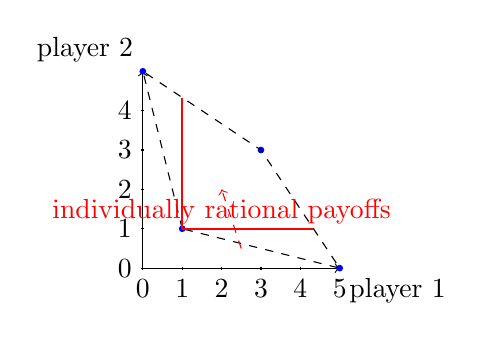
\begin{tikzpicture}[scale=0.5]
        \draw[->] (0,0) -- (5,0) node[anchor=north west] {player 1};
        \draw[->] (0,0) -- (0,5) node[anchor=south east] {player 2};
        \foreach \x/\xtext in {0,1,2,3,4,5}
            \draw (\x cm,1pt) -- (\x cm,-1pt) node[anchor=north] {$\xtext$};
        \foreach \y/\ytext in {0,1,2,3,4}
            \draw (1pt,\y cm) -- (-1pt,\y cm) node[anchor=east] {$\ytext$};
        \filldraw [blue] (1, 1) circle (2pt);
        \filldraw [blue] (0, 5) circle (2pt);
        \filldraw [blue] (5, 0) circle (2pt);
        \filldraw [blue] (3, 3) circle (2pt);
        \draw[black, dashed] (1,1) -- (0,5) -- (3,3) -- (5,0) -- (1,1);
        \draw[red, thick] (1, 1) -- (1, 13/3);
        \draw[red, thick] (1, 1) -- (13/3, 1);
        \draw[red, dashed, ->] (2.5, 0.5) -- (2, 2) node[anchor=north]{individually rational payoffs};
    \end{tikzpicture}
    \caption{A plot highlighting the possible individually rational payoffs for the game of A Prisoner's Dilemma.}\label{fig:Feasible_Payoff_Plot}
\end{figure}

In the next section (Section~\ref{sec:Folk_Thm}), the main theorem of this
project will be stated and proved.

\section{Folk Theorem}\label{sec:Folk_Thm}
According to~\cite{Webb2007}, the class of theorems known as Folk Theorems are
so-called because the result was well-known before a formal proof was provided.
In general, these theorems state that players can achieve a better payoff than
the Nash equilibrium (if the Nash equilibrium payoff is not optimal) when the
stage game is repeated many times and the probability of the game continuing is 
large enough. 

It is believed that Friedman, 1971 (~\cite{friedman1971non}) was one of the
first to publish a formal proof to the widely accepted Folk Theorem~\cite{}.
Thus, the presentation of the statement and proof given here is adapted
from~\cite{friedman1971non} as well as from~\cite{Knight2017b}.

Before stating the theorem, the list of assumptions which
Friedman~\cite{friedman1971non} requires the infinite repeated game to satisfy is given.
\begin{enumerate}
    \item The mixed action sets, \(\Sigma_{i}\) are compact and convex for all
    \(i\in N\). 
    \item The payoff functions, \(U_{i}: \Sigma \to \mathbb{R}\), are continuous
    and bounded for all \(i\in N\).
    \item The \(U_{i}(\sigma)\)s are quasi-concave~\footnote{According
    to~\cite{Stover}, a real-valued function \(f\), defined on a convex subset
    \(C \subset \mathbb{R}^n\), is \textit{quasi-concave} if for all \(\alpha
    \in \mathbb{R}\), the set \( \{ x \in C : f(x) \ge a \} \) is convex.}
    functions of \(sigma_{i}\) for all \(i\in N\).
    \item If  \(U_{i}^{\prime} \le U_{i}^{\prime\prime}\), for all \(i\in N\)
    and \(U_{i}^{\prime}, U_{i}^{\prime\prime} \in H\), then, for all
    \(U_{i}^{\prime} \le U \le U_{i}^{\prime\prime}\), \(U \in H\). Here, \(H\)
    is defined to be the set of feasible payoffs, \( \{ U(\sigma) : \sigma \in
    \Sigma \} \), where \(U(\sigma) = (U_{1}(\sigma), U_{2}(\sigma), \ldots,
    U_{N}(\sigma))\).
    \item  \(H^{*}\) is concave, where \(H^{*} \subset H\) denotes the set of
    all Pareto optimal payoffs.~\footnote{Friedman defines a \textit{Pareto
    optimal payoff} as a point in the payoff space \(U_(\sigma^{*})\) which
    satisfies the conditions: \(\sigma^{*} \in \Sigma \) and \(U_{i}(\sigma^{*})
    > U_{i}(\sigma)\) for all \(i \in N\)}.
    \item All stage games are identical in the infinitely repeated game.
    \item The discount parameter, \(\delta \), is equal in all time periods.
    \item The stage game has a unique Nash equilibrium.
    \item The Nash equilibrium is not Pareto optimal. 
\end{enumerate}
Note, Friedman~\cite{friedman1971non} later goes on to prove that assumptions
six to nine can be removed with only a small effect on the result. However,
since the only game being studied in this project is the IPD (which satisfies
all the above assumptions), this generalisation will be omitted. Thus, only the
proof of the original theorem will be provided.

\begin{theorem}\label{thm:Folk}
    If the above assumptions are all satisfied for the given infinite repeated
    game, then for any individually rational payoff \(V_{i}\) (greater than the
    payoff yielded by the stage Nash equilibrium \(\sigma^{ne}\)), there exists
    a discount parameter \(\delta^{*}\) such that for all \(\delta_{i}\), \(0 <
    \delta^{*} < \delta_{i} < 1\) there is a subgame perfect Nash equilibria
    with payoffs equal to \(V_{i}\).
\end{theorem}

\begin{proof}
    Consider the set of all actions which yield greater payoffs than the Nash
    equilibrium, denoted by:
    \[
        B = \{\sigma : \sigma \in \Sigma, U_{i}(\sigma) > U_{i}(\sigma^{ne}), i = 1, 2, \ldots, N\}
    \]
    and define the following trigger strategy:
    \begin{equation}
        \sigma_{i1} = \sigma_{i}^{\prime}, \newline
        \sigma_{it} = \begin{cases}
            \sigma_{i}^{\prime}, & \quad \text{if } \sigma_{j\tau}=\sigma_{j}^{\prime} \ j \ne i, \tau=1, 2, \ldots, t-1, t=2, 3, \ldots \\
            \sigma_{i}^{ne}, & \quad \text{otherwise},
        \end{cases}
    \end{equation}\label{eqn:trigger_strategy}
    where \(\sigma_{i}^{\prime} \in B\). In words, the \(i\)th player will choose \(\sigma_{i}^{\prime}\) unless any
    other player does not play \( \sigma_{j}^{\prime}\), in which case they
    continue by playing their Nash equilibrium action, \(\sigma_{i}^{ne}\). Now,
    by definition, the strategy in~\ref{eqn:trigger_strategy} is an equilibrium
    of the repeated game if 
    \[
        \sum_{\tau=0}^{\infty}{\delta_{i}^{\tau}U_{i}(\sigma_{i}^{\prime})} > U_{i}(\sigma_{-i}^{\prime}, t_{i}) + \sum_{\tau=1}^{\infty}{\delta_{i}^{\tau}U_{i}(\sigma^{ne})}, \ \ i=1, 2, \ldots, N,
    \]
    which can be rearranged to 
    \[
        \frac{\delta_{i}}{1-\delta_{i}}[U_{i}(\sigma^{\prime}) - U_{i}(\sigma^{ne})] > U_{i}(\sigma_{-i}^{\prime}, t_{i}) - U_{i}(\sigma{\prime}), \ \ i=1, 2, \ldots, N,
    \]
    where \(U_{i}(\sigma_{-i}^{\prime}, t_{i}) = \max_{\sigma_{i} \in
    \Sigma_{i}}{U_{i}(\sigma_{-i}^{\prime}, \sigma_{i})}\), \(t_{i} \in
    \Sigma_{i}\).

    To check if this strategy is indeed a best response to all others players,
    who are executing the same strategy in~\ref{eqn:trigger_strategy}, for the
    \(i\)th player consider their alternatives. They have two options: either
    the \(i\)th player executes the strategy in question, or they play the
    strategy in which \(\sigma_{i1} = t_{i}\) and then \(\sigma_{i\tau} =
    \sigma^{ne}\) will be the best response as every other player will convert
    to \(\sigma_{j\tau} = \sigma^{ne}\), for all \(\tau > 1\). Note that any
    other strategy is weakly dominated by one of these two, since playing
    \(t_{i}\) in any other stage \(\tau \ne 1\) will yield less gains as these
    stages have increased discounting.

    Now, if the discounted loss from playing the Nash equilibria,
    \begin{equation}
        \frac{\delta_{i}}{1-\delta_{i}}[U_{i}(\sigma^{\prime}) -
        U_{i}(\sigma^{ne})],
    \end{equation}\label{eqn:discounted_loss}
    is greater than the gain achieved by playing
    \(t_{i}\) against \(\sigma_{-i}^{\prime}\), then the rational
    strategy choice for player \(i\), assuming all other players are
    executing~\ref{eqn:trigger_strategy}, is to play~\ref{eqn:trigger_strategy}.
    
    Observe, as the discount parameter, \(\delta \), tends to one from
    below, the discounted loss in~\ref{eqn:discounted_loss} tends to infinity.
    However, the gain obtained from playing \(t_{i}\), that is,
    \(U_{i}(\sigma_{-i}^{\prime}, t_{i}) - U_{i}(\sigma{\prime})\) is finite.
    Thus, for all \(\sigma_{i}^{\prime} \in B\) there exists a \(\delta^{*} \in
    (0, 1)\) such that for all \(\delta_{i} > \delta^{*}\), the
    strategy~\ref{eqn:trigger_strategy} is optimal against the same strategy for
    all players \(j \ne i\). Therefore, if the conditions are true for all
    players \(i = 1,2,\ldots,N\), the strategy \((\bar{\sigma}_{1},
    \bar{\sigma}_{2}, \ldots, \bar{\sigma}_{N})\), where  \(\bar{\sigma}_{i}\)
    denotes~\ref{eqn:trigger_strategy}, yields a Nash equilibrium.

    Finally, by construction, the strategy~\ref{eqn:trigger_strategy} is indeed
    a subgame perfect equilibrium. 
\end{proof}

\section{Aims of the Project}\label{sec:Aims_of_the_Project}
This project stemmed from an initial idea used in Game Theory Coursework
written by the author. In this coursework, regarding Nash equilibria and
repeated games, the two graphs, as presented in Figure~\ref{fig:CW_plots}, were
obtained.

%\begin{figure}[h]
%    \centering
%        \begin{subfigure}[t]{0.45\textwidth}
%        \centering
%        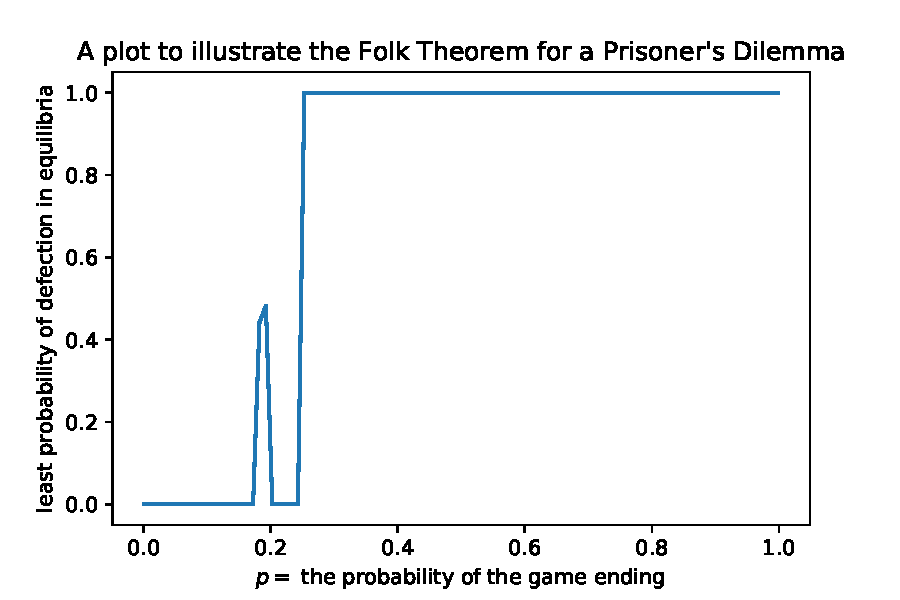
\includegraphics[width=\linewidth]{CW-graph-1.pdf}
%        \caption{A plot of the least probabilities of defection when playing %against the strategies: Cooperator, TitForTat and Random. Here, the %p-threshold is approximately 0.25.}\label{fig:CW_graph_1}
%        \end{subfigure}
%    \hfill
%        \begin{subfigure}[t]{0.45\textwidth}
%        \centering
%        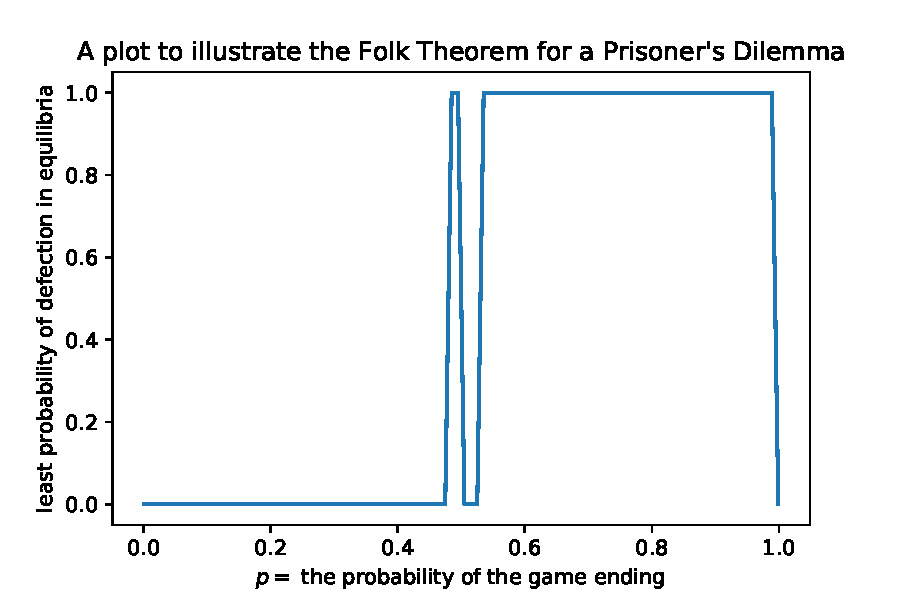
\includegraphics[width=\linewidth]{CW-graph-2.pdf}
%        \caption{A plot of the least probabilities of defection when playing %against the strategies: Winner21, AntiTitForTat and OmegaTFT.\@ Here, %the p-threshold is around 0.5.}\label{fig:CW_graph_2}
%        \end{subfigure}
%        \caption{Original plots obtained which inspired the creation of this %project.}\label{fig:CW_plots}
%\end{figure}

These two graphs were obtained using a similar method to this project and so see Chapter~\ref{ch:Methods_Init_Investigations} for the details. The
plots show the least probability of defection obtained in the Nash equilibria of
the game. The game matrices were defined by repeating an IPD tournament 100
times for the Defector strategy, and three other opponents, with 100 distinct
probabilities of the game ending.

From Figure~\ref{fig:CW_plots}, it can be seen that there appears to be a `clear
probability' of the game ending at which the least probability of defection
jumps from zero to one. (Throughout the rest of this project, this `clear
probability', \(p\), will be referred to as the \emph{p-threshold} of a game.)
However, what was most intriguing was that the two different games obtained had
a different p-threshold (approximately 0.25 for Figure~\ref{fig:CW_graph_1} but
for Figure~\ref{fig:CW_graph_2} the threshold appears at around 0.5). This
inspired the idea to investigate whether there are any specific characteristics
of an IPD tournament that affect the value of this threshold. That is, does the
number or the stochasticity of players, for example, cause the probability of a
game ending for which the least probability of defection jumps to increase or
decrease?

Therefore, the aims of this project are as follows:
\begin{enumerate}
\item To look thoroughly into the recent (and past) literature of
research already produced in the areas of Folk Theorems and the IPD;\@
\item To execute a large experiment involving many tournaments of the
IPD with different types / numbers of players to obtain graphs similar
to those in Figure~\ref{fig:CW_plots};
\item To perform analyses on where the p-thresholds seem to lie and
whether it is affected by the different environments of the tournaments
(that is, differing number of players, stochasticity within the
tournament itself and the players, etc.); and
\item To explore other `Folk-like' Theorems and perform similar
experiments and analyses.  
\end{enumerate}
